\section{Como a máquina aprende}
\label{sec:howdoesmachinelearn}

O processo básico de aprendizagem de máquina consiste em entrada de dados, abstração e generalização (Figura~\ref{fig:processo-aprendizagem}).
\begin{alineas}
	\item Entrada de dados: são fatos tirados da memória ou da observação;
	\item Abstração: transformar estes dados em algo mais objetivo e que faça sentido; e
	\item Generalização: utiliza os dados abstraídos para identificar padrões e assim classificá-los.			
\end{alineas}

\begin{figure}[h!]
	\centering
	\Caption{\label{fig:processo-aprendizagem} Fluxo do processo de aprendizagem.}	
	\UECEfig{}{
		\fbox{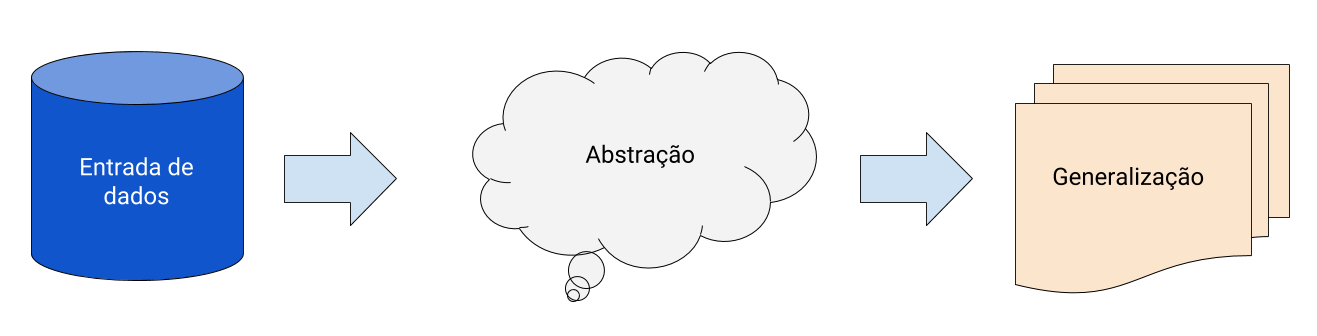
\includegraphics[width=15cm]{figuras/procc-learning}}
	}{
		\Fonte{Autoria própria.}
	}	
\end{figure}

Todo este processo ocorre na ordem apresentada, pois o conceito de abstração e generalização estão muito próximos e tecnicamente um não faz sentido sem o outro. Os passos de abstração e generalização do processo de aprendizagem ocorrem subconscientemente em seres humanos, logo pode ser complexo representar este processo em linguagem computacional.


\subsection{Abstração e Representação de Dados}
\label{subsec:abs-representacao-dados}

Durante a abstração os dados de entradas, são preparados para que possuam algum sentido em um contexto.
Para ilustrar este processo, lembre de quando aprendeu a executar operações de soma e subtração, que sua professora apresentou (Figura ~\ref{fig:exemplo-aprendizagem}).

\begin{figure}[ht!]
	\centering
	\Caption{\label{fig:exemplo-aprendizagem} Uma maçã mais outra maçã é igual à duas maçãs.}	
	\UECEfig{}{
		\fbox{
\includegraphics[width=15cm]{figuras/exemplo_soma_maca}}
	}{
		\Fonte{Autoria própria.}
	}	
\end{figure}

Você ignorou todas as propriedades da maçã como ser uma fruta, ter a cor vermelha  ou possuir sementes, e focou nas propriedades que faziam sentido no contexto, que é a maçã representar uma unidade. Logo uma unidade de um tipo mais outra unidade do mesmo tipo é igual à duas unidades, ou seja para o contexto de soma não importa se é uma fruta ou a cor e sim a unidade. Após o processo de abstração formou-se ideia apresentada na \autoref{fig:exemplo-aprendizagem2}.


\begin{figure}[ht!]
	\centering
	\Caption{\label{fig:exemplo-aprendizagem2} Exemplo soma com maçãs após o processo de abstração.}	
	\UECEfig{}{
		\fbox{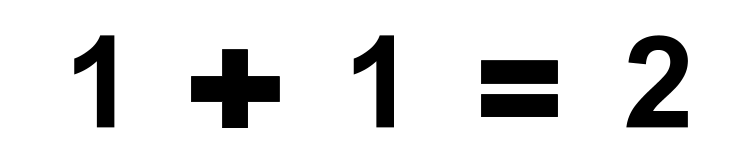
\includegraphics[width=15cm]{figuras/exemplo_soma_maca2}}
	}{
		\Fonte{Autoria própria.}
	}	
\end{figure}

A etapa seguinte do processo de abstração é a representação do conhecimento, onde é gerado um 
\textbf{\textit{modelo}} 
Existem vários tipos de modelos, alguns deles são:
\begin{alineas}
    \item equações;
    \item grafos; e
    \item estruturas de lógicas de programação como: \textit{if} e \textit{else}. 
\end{alineas} 

A escolha do modelo não é feita pelo sistema de aprendizagem, depende do tipo da tarefa \textbf{\textit{T}} e o tipo dos dados
que estão sendo analisados. A etapa que gera um modelo específico de um conjunto de dados é chamada de treino de dados \textbf{\textit{E}}. 
Durante o treinamento, os dados são transformado em uma forma abstrata que resume os dados originais, é importante observar que o  
treino de dados não gera novos dados, muitas vezes após esta etapa nos surpreendemos com as suposições levantadas sobre como 
estes dados se relacionam. Estas relações identificadas sempre estiveram presente, porém quando se organiza estes dados de outra forma
é possível identificar estas conexões escondidas.

\subsection{Generalização}
\label{subsec:generalização-dados}

Até que o sistema possa utilizar o conhecimento abstrato para uma ação futura, o processo de aprendizagem ainda não está concluído.
O processo de generalização transforma o conhecimento abstrato prévio em um formato que possa ser utilizado para um ação, é um 
processo difícil de ser descrito, mas pode ser visto como uma busca nos modelos ou teorias geradas no processo de abstração, porém pode existir
um grande número de modelos disponíveis.

Dado que exista um grande número de modelos, durante a generalização este número será reduzido de forma qualitativa. 
Mas não é praticável examinar cada um dos modelos e verificar se atende aos parâmetros, portanto os algoritmos de machine learning utilizam 
técnicas de busca como heurística para diminuir a área de busca para encontrar os modelos que mais se aproximam do esperado.
Segundo \cite{heuristica}:
\begin{citacao}
A pesquisa por heurísticas é uma pesquisa realizada por meio da quantificação de proximidade a um determinado objetivo. 
Diz-se que se tem uma boa (ou alta) heurística se o objeto de avaliação está muito próximo do objetivo; diz-se de má (ou baixa) heurística 
se o objeto avaliado estiver muito longe do objetivo. 
Etimologicamente a palavra heurística vem da palavra grega Heuriskein, que significa descobrir (e que deu origem também ao termo Eureca).
\end{citacao} 


Porém como a heurística trabalha com proximidade, não há garantias de que os melhores modelos serão escolhidos, 
no entanto é impraticável realizar esta pesquisa sem utilizar está técnica.

\subsubsection{Avaliando o sucesso da aprendizagem}
\label{subsec:avaliando-generalização-dados}

A heurística aplicada em aprendizagem de máquina as vezes resulta em modelos errados, se os modelos constantemente 
forem imprecisos, é necessário incluir tendências no algoritmo e utilizar técnicas estatísticas como \textbf{bias} e \textbf{variância} 
para identificar os erros. Porém é necessário atentar para que estes ajustes não deturpem a realidade e acabe causando o \textit{overfitting}.
Por exemplo dado um algoritmo que identifica rostos em imagens, ele procura por dois circulos (os olhos) em cima de uma linha (a boca), isto pode 
ser considerado uma tendência, ao treinar os modelos será utilizado varias imagens com diversas formas de rosto, com óculos, 
com barba, olhando para o lado, etc.
Após o treino teremos vários outros modelos para a mesma finalidade, logo devemos poder medir o quanto estes modelos 
se diferenciam da tendência e entre si. Neste caso conseguimos ter dois parâmetros de erro de modelo:

\begin{alineas}
	\item Bias: é a diferença entre o valor das tendências e os valores reais. Em suma bias está relacionado a capacidade de um modelo
				se ajustar aos dados; e
	\item Variância: é a variabilidade dos modelos. Está relacionada a capacidade do modelo se ajustar à novos dados.  
\end{alineas}   

Matematicamente, se nossa função real é \textit{Y = f(X) + E}, e queremos estimar um modelo \textit{h(x)} que aproxima a função \textit{f(x)},
o bias (1) e a variância (2) serão, respectivamente na (Figura~\ref{fig:bias-func}).

\begin{figure}[ht!]
	\centering
	\Caption{\label{fig:bias-func} Modelo matemático: Bias e Variância}	
	\UECEfig{}{
		\fbox{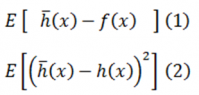
\includegraphics[width=10cm]{figuras/bias-variance}}
	}{
		\Fonte{https://ericcouto.wordpress.com/2013/06/29/bias-vs-variancia-parte-1 (2013).}		
	}	
\end{figure}

A última etapa da generalização é determinar o sucesso dos modelos, depois de treinado com os dados iniciais
o modelo é testado com novos dados e avaliado como o processo de generalização se comporta, é importante saber que é extremamente raro
que um modelo atenda perfeitamente todos os casos imprevistos.
Um dos motivos para que um modelo não generalize perfeitamente todos os casos é chamado de ruído, são variações não previstas nos dados.
Estes ruídos são causados por dados corrompidos, cálculos imprecisos ou até mesmo entrada de dados inconsistentes.









 